\documentclass{article}
\usepackage[utf8]{inputenc}
\usepackage[T1]{fontenc}
\usepackage[english]{babel}
\usepackage{mathtools}
\usepackage{physics}
\usepackage{amsthm}
\usepackage[left=3cm, top=3cm, right=2cm, bottom=2cm, a4paper]{geometry}
\usepackage{anyfontsize}
\usepackage{array}
\usepackage{booktabs}
\usepackage{natbib}
\usepackage{csquotes}
\usepackage{indentfirst}
\usepackage{fancyhdr}
\usepackage{amsmath, amssymb, graphicx, caption, subcaption, booktabs}
\usepackage{pgfplots}
\usepackage{tikz}
\pgfplotsset{compat=1.18}
\usepackage{float}
\usepackage{siunitx} % For decimal alignment
\usepackage{pdfpages} 

% Hyperref should be loaded LAST
\usepackage[colorlinks=true, linkcolor=blue, citecolor=blue, urlcolor=blue]{hyperref}

\setlength{\parindent}{1.25cm}

% ABNT-style page numbering (right-aligned in footer)
\pagestyle{fancy}
\fancyhf{}
\fancyfoot[R]{\thepage}
\renewcommand{\headrulewidth}{0pt}

\title{Western Relationship, China and Taiwan: \\ An Econometric Approach to Assess Tensions}
\author{
    Alison Cordeiro Sousa\textsuperscript{1} \\
    Alexandre Ratsuo Uehara\textsuperscript{2} \\
    Rodrigo Cintra\textsuperscript{3}
}
\date{}

\begin{document}
\fontsize{12pt}{18pt}\selectfont

\begin{center}
{\LARGE \textbf{Western Relationship, China and Taiwan: \\ An Econometric Approach to Assess Tensions}}

\vspace{1.5cm}

\textbf{Alison Cordeiro Sousa}\footnote{Bachelor’s Candidate in International Relations, Escola Superior de Propaganda e Marketing (ESPM).}\\
Escola Superior de Propaganda e Marketing (ESPM)\\
Dr. Álvaro Alvim, 123\\
04018-010 – São Paulo, SP – Brazil\\
\texttt{alison.sousa@acad.espm.br}

\vspace{1cm}


\textbf{Rodrigo Cintra}\footnote{Professor of International Relations, Ph.D. in International Relations, University of Brasília (UnB).}\\
Escola Superior de Propaganda e Marketing (ESPM)\\
Dr. Álvaro Alvim, 123\\
04018-010 – São Paulo, SP – Brazil\\
\texttt{cintra@espm.br}

\vspace{1.5cm}

October 4, 2024
\end{center}

\thispagestyle{empty} % Remove número da primeira página

\newpage

\section*{Abstract}
This research project examines the economic dimensions of China–U.S.–Taiwan tensions between 2012 and 2022, focusing on trade flows, foreign direct investment, and regional integration. Using international trade theory and spatial econometrics, the research analyzes Taiwan’s economic dependence on China, the asymmetry in investment patterns, and the impacts of trade agreements such as ASEAN+1. Results indicate that Taiwan’s exclusion from key regional frameworks undermines its competitiveness, while growing U.S.–China rivalry reshapes trade and investment dynamics across East Asia.

\vspace{0.5cm}
\noindent\textbf{Keywords:} International Trade; China; Taiwan; Regional Integration; Spatial Econometrics; East Asia.

\section{Introduction}

The Republic of China (ROC), or Taiwan, is an island located 200 km from the People's Republic of China (PRC), governed independently and recognized as a sovereign state by 20 nations worldwide \citep{barbosa_who_cares_about_taiwan}. The PRC considers the island a rebellious province that is part of its territory \citep{vladimir_ivanov_rebel_island_china_taiwan_question}. Russia's occupation of Ukraine, beginning on February 24, 2022, with tacit support from China for the invasion, has fueled speculations within the international system regarding Beijing's intentions toward Taiwan \citep{yeung_what_you_need_to_know_china_taiwan_tensions}. For instance, \citet{tadeu_brazil_vote_resolution} suggests that China's abstention from voting in the United Nations Security Council on a resolution condemning Russia raised global concerns about the possibility of a Chinese attack on the island.

Furthermore, it has been observed that over the past few decades, the United States has sought to enhance Taiwan's involvement in the international system concerning trade and security \citep{wenzhao_taiwan_policy_obama_administration}. China perceives this effort as an action that exacerbates tensions with Taiwan, potentially necessitating the use of force to assert control over the island \citep{hernandez_china_suspends_diplomatic_contact, trent_chinas_views_of_regional_security}.

In this context, Chinese assertions of a singular China in the region view such actions as violations of their sovereignty. Conversely, the U.S. Congress upholds its commitment to supporting Taiwan's vibrant democracy. Therefore, according to \citet{hsu_cross_strait_peace_development}, the complexity of relations between both sides of the Taiwan Strait cannot be portrayed solely from a political or security perspective; it also warrants an economic approach to better understand the levels of tension between these nations. Given that their foreign trade is significantly intertwined, with China accounting for over \$82 billion and the United States approximately \$40 billion of Taiwan's trade, it is essential to analyze these aspects \citep{ma_trade_balance_china_taiwan}.

Since foreign trade and national security are closely linked, metrics such as spatial econometrics can facilitate the research process to statistically assess whether rising tensions on both sides of the Strait may be increasing or decreasing the percentage of Chinese investments in the Taiwanese market \citep{pietrafesa_political_economic_relations_china_taiwan_usa}. Overall, it is evident that Chinese hostility toward Taiwan is intensifying, largely due to Taiwan's increasing westernization \citep{tian_china_drops_peaceful_in_push_for_taiwan_reunification}. Consequently, this may also result in a reduction of Taiwanese investments in Mainland China \citep{yeung_what_you_need_to_know_china_taiwan_tensions}.

Spatial econometric analysis reveals how Taiwan's closer ties with the United States affect the island's investment and trade strategies with China. Essentially, Taiwanese investments in China and business risks are negatively correlated, indicating that Taiwan's investments have been influenced by the overall economic relations between the two nations, particularly amidst heightened tensions in recent years \citep{gomes_international_trade_per_capita_gdp}. This dynamic also impacts business strategies for companies based in Taiwan.

Thus, the aim of this research project is to examine and evaluate the levels of tension among the United States, China, and Taiwan between 2012 and 2022, as well as the reasons behind the escalation of tensions during these periods, addressing both security and economic relations.

Finally, the research project intends to explore the following themes: the economic relationships among China, Taiwan, and the United States. The objective is to ascertain the extent to which the Chinese government is willing to employ political or economic force for the reunification of both sides of the Taiwan Strait and to analyze the posture of American policies toward both Chinese and Taiwanese entities.

\section{The Advancement of International Economy Among China, United States, and Taiwan}

This section examines Taiwan's foreign trade dynamics within the context of its complex economic relationships with China and the United States. We analyze the structural implications of Taiwan's exclusion from the ASEAN Agreement and employ spatial econometric methods to assess how geopolitical tensions influence cross-strait investment patterns.

\subsection{Taiwan's Foreign Trade: Dependence on China and the United States Under Krugman's Trade Policy Framework}

The triangular economic relationship between China, the United States, and Taiwan represents a paradigmatic case of strategic interdependence in global trade networks. Taiwan's export-oriented economy exhibits pronounced dependence on both major powers: China accounted for \$82 billion (24\% of total trade) and the United States \$40 billion (12\%) in 2021 \cite{ma_trade_balance_china_taiwan, bureau_of_trade_exports_imports_2022}. This asymmetric integration manifests most visibly in the persistent trade imbalance with China, which accumulated a \$140 billion deficit with Taiwan from 2015-2020 (Figure \ref{fig:tradebalance}).


\begin{figure}[h]
    \caption{Trade balance between China and Taiwan (2015–2020)}
    \centering
    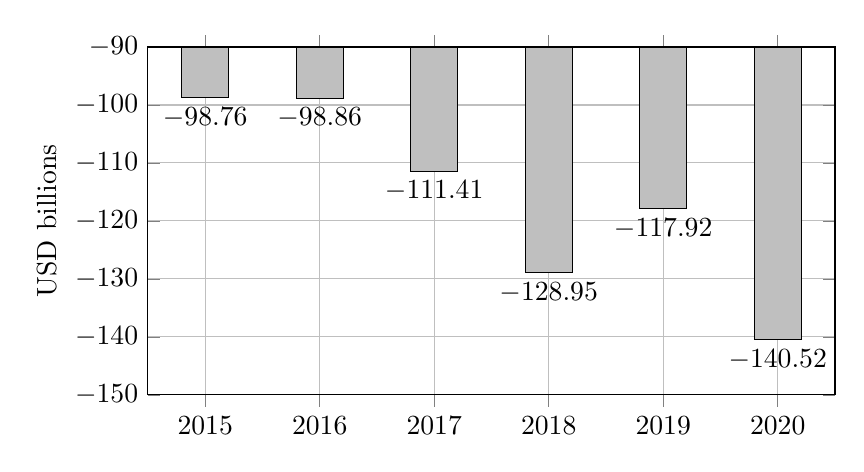
\begin{tikzpicture}
        \begin{axis}[
            ylabel={USD billions},
            ymin=-150, ymax=-90,
            xtick={2015,...,2020},
            ytick={-150,-140,...,-90},
            grid=major,
            width=0.85\textwidth,
            height=6cm,
            ybar,
            bar width=0.6cm,
            symbolic x coords={2015,2016,2017,2018,2019,2020},
            nodes near coords={\pgfmathprintnumber[precision=2]{\pgfplotspointmeta}},
        ]
        \addplot[fill=gray!50] coordinates {
            (2015,-98.76) (2016,-98.86) (2017,-111.41)
            (2018,-128.95) (2019,-117.92) (2020,-140.52)
        };
        \end{axis}
    \end{tikzpicture}
    \caption*{Source:  Adapted from \cite{ma_trade_balance_china_taiwan}.}
    \label{fig:tradebalance}
\end{figure}


The semiconductor industry epitomizes this interdependence. According to \cite{zandt_who_relies_on_taiwanese_trade}, Taiwan supplies 62\% of U.S. semiconductor imports, with leading firms like Apple and NVIDIA dependent on TSMC's advanced foundries. However, as noted by the \cite{us_department_state_biden_sotu} the Biden administration's “friendshoring” strategy, together with Intel’s \$20 billion investment in semiconductor manufacturing plants in Ohio, according to \cite{king_intel_chip_hub}, signals growing pressures for strategic decoupling that may reshape existing trade relationships.

This policy orientation is further underscored by the phrase \textit{``producing for the Americans,''} mentioned in President Joe Biden's 2022 State of the Union address regarding the international market, underscores the geopolitical complexities in the China-Taiwan-U.S. triangular relationship. A significant portion of U.S. industrial supply chains operates across both regions, by the \cite{us_department_state_biden_sotu}. Biden's remarks signal a strategic shift toward \textit{``friendshoring''}—relocating production to allied nations while reshoring critical industries. For instance:
\begin{itemize}
    \item Macy's announced plans to diversify production outside China.
    \item Intel pledged \$20 billion to build semiconductor fabrication plants near Columbus, Ohio, aiming to surpass Taiwan's global chip dominance.
\end{itemize}
These developments will inevitably reshape trade dynamics among these economies.

A second critical factor is tariff policy. The \textit{ASEAN-China Free Trade Agreement} (ACFTA, enacted January 1, 2010) eliminated or reduced tariffs on over 90\% of traded goods between China and ASEAN member states, as emphasized by \cite{feddersen_china_strategies_towards_taiwan}. Taiwan's exclusion from this framework exacerbates its trade asymmetry with China.

\subsection{Structural Disadvantages: Taiwan's Exclusion from ASEAN+1}

The ASEAN-China Free Trade Agreement (ACFTA), implemented in 2010, created a preferential trade regime that systematically disadvantages non-member economies. This creates a competitive asymmetry that \cite{chou_economy_cooperation_framework_agreement} warns could lead to Taiwan's "economic marginalization" in three ways:

\begin{enumerate}
    \item Divestment of Taiwanese firms from China to circumvent tariff disadvantages
    \item Hollowing-out of domestic industries through reduced FDI (estimated 29-42\% decline)
    \item Market share erosion to South Korea, which enjoys both ASEAN+3 privileges and technological parity
\end{enumerate}

\subsection{Welfare Analysis of Trade Policy Distortions}

Applying Krugman's trade policy framework \cite{krugman_obstfeld_international_economics}, we model the welfare effects of Taiwan's tariff disadvantages (Figure \ref{fig:krugman}). The standard partial equilibrium analysis decomposes impacts into:

\begin{figure}[h]
    \caption{Deadweight loss (b+d) vs. terms-of-trade gain (e)}
    \centering
    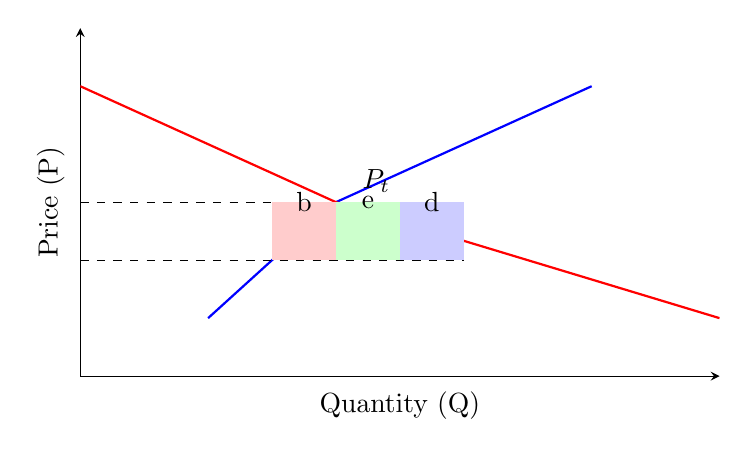
\begin{tikzpicture}
        \begin{axis}[
            axis lines=left,
            xlabel={Quantity (Q)},
            ylabel={Price (P)},
            xtick=\empty, ytick=\empty,
            width=0.8\textwidth,
            height=6cm,
            xmin=0, xmax=10,
            ymin=0, ymax=6,
        ]
        % Economic curves
        \addplot[blue, thick] coordinates {(2,1) (4,3) (8,5)}; % Supply
        \addplot[red, thick] coordinates {(0,5) (4,3) (10,1)}; % Demand
        % Price lines
        \addplot[dashed, black] coordinates {(0,2) (6,2)} node[above left]{$P_w$};
        \addplot[dashed, black] coordinates {(0,3) (5,3)} node[above left]{$P_t$};
        % Areas
        \addplot[fill=green!20, draw=none] coordinates {(4,2) (4,3) (5,3) (5,2)} node[pos=0.5]{e};
        \addplot[fill=red!20, draw=none] coordinates {(3,2) (3,3) (4,3) (4,2)} node[pos=0.5]{b};
        \addplot[fill=blue!20, draw=none] coordinates {(5,2) (5,3) (6,3) (6,2)} node[pos=0.5]{d};
        \end{axis}
    \end{tikzpicture}
    \caption*{Source: Adapted from \cite{krugman_obstfeld_international_economics}.}
    \label{fig:krugman}
\end{figure}



The net welfare effect follows:
\[
\Delta W = \underbrace{-(b + d)}_{\text{Efficiency loss}} + \underbrace{e}_{\text{Trade gain}}
\]

For Taiwan's small open economy, the terms-of-trade gain (e) proves negligible while distortionary losses (b+d) dominate. Table \ref{tab:tradepolicy} summarizes how these welfare effects manifest across different policy instruments. Three key observations emerge from this analysis: First, all protectionist measures uniformly benefit domestic producers at consumers' expense. Second, the welfare calculus becomes particularly adverse for small economies like Taiwan, where the deadweight losses (triangles b+d) outweigh any potential terms-of-trade gains (rectangle e). Third, the revenue implications vary substantially - while tariffs generate government income, quotas and VERs simply transfer rents to license-holders or foreign firms. This suggests that for economies facing political constraints on regional trade integration, tariff measures may dominate other instruments when revenue generation is prioritized, though all options remain Pareto-suboptimal compared to free trade benchmarks.

\begin{table}[h]
    \centering
    \caption{Comparative Effects of Trade Policy Instruments}
    \begin{tabular}{@{}lp{2cm}p{2cm}p{2cm}p{2cm}@{}}
    \toprule
    \textbf{Policy Effect} & \textbf{Import Tariff} & \textbf{Export Subsidy} & \textbf{Import Quota} & \textbf{VER} \\ 
    \midrule
    Producer Surplus & Increases & Increases & Increases & Increases \\ 
    \addlinespace[0.3cm]
    Consumer Surplus & Decreases & Decreases & Decreases & Decreases \\
    \addlinespace[0.3cm]
    Government Revenue & Increases & \raggedright Decreases (gov. spending $\uparrow$) & No change (licenses) & No change (foreigners) \\
    \addlinespace[0.3cm]
    National Welfare & \raggedright $\downarrow$ (small economy) & Decreases & \raggedright $\downarrow$ (small economy) & Decreases \\ 
    \bottomrule
    \end{tabular}
    \caption*{Source: Compiled by the author.}
    \label{tab:tradepolicy}
\end{table}

Table \ref{tab:tradepolicy} reveals three critical patterns for Taiwan's economy: First, all four policies show identical distributional effects - producers gain (row 1) while consumers lose (row 2). Second, only tariffs improve government revenue (row 3), with subsidies being fiscally costly. Third, welfare consistently declines (row 4), with tariffs and quotas being particularly damaging for small economies. This uniform welfare loss confirms that Taiwan's minimal terms-of-trade gains (e) cannot offset the substantial deadweight losses (b+d) shown in the table's welfare row. The revenue column explains why tariffs might be politically preferred despite identical welfare outcomes to quotas/VERs.

Finally, even though the United States is involving Taiwan in trade and international affairs, it is observed that in the coming decades, the island may not maintain as strong a trade connection with the United States due to American investments in semiconductor chip production in Columbus as noted by \cite{king_intel_chip_hub}. Meanwhile, China is increasingly attempting to isolate Taiwan from regional trade and the rest of the world, according to \cite{feddersen_china_strategies_towards_taiwan}. One possible response from Taiwan is to reduce its investments in mainland China, as there is a notable lack of significant correlation in some regions regarding Taiwanese investments in Chinese trade.

\subsection{Spatial Econometric Modeling of Cross-Strait Economic Relations}

The increasing assertiveness of China’s foreign policy toward Taiwan, particularly under Xi Jinping’s administration, has underscored the necessity for rigorous econometric analysis capable of capturing the complex spatial and temporal dimensions of cross-Strait economic interactions. In this context, spatial econometric modeling emerges as a crucial methodological approach to evaluate how Taiwan’s investment and trade behavior toward mainland China has evolved, especially in light of the growing geopolitical divergence under President Tsai Ing-wen, whose administration has consistently demonstrated a West-leaning orientation \citep{tian_china_drops_peaceful_in_push_for_taiwan_reunification}.

To quantify the implications of China’s political assertiveness, prior analyses have employed logistic regressions to demonstrate that the probability of a hostile diplomatic response from Taiwan increases substantially—up to 53.10 times—when Chinese diplomatic posture is itself aggressive \citep{pietrafesa_political_economic_relations_china_taiwan_usa}. While these findings underscore behavioral correlations, they do not fully encapsulate the underlying spatial dynamics. Therefore, to rigorously analyze the heterogeneity and spatial dependence within Taiwanese investments in China, we turn to spatial econometric techniques such as Moran’s I, spatial autoregressive models (SAR), and spatial error models (SEM).

The Moran’s I index serves as a foundational tool to detect spatial dependence and heterogeneity in panel data over geographical regions. It measures the similarity of an attribute among neighboring regions and provides a global test of spatial autocorrelation. The index takes values in the bounded interval $-1 \leq I \leq 1$: positive values imply positive spatial autocorrelation (neighboring regions exhibit similar behavior), negative values indicate spatial repulsion (dissimilar behavior), and a value near zero suggests spatial randomness or independence.

Global and local versions of Moran’s I are computed to capture broad spatial structures and localized clusters of investment behavior. This research utilizes investment data provided by Taiwan's Ministry of Economic Affairs, covering 21 provincial units across mainland China, including Beijing, Shanghai, Guangdong, Jiangsu, and Sichuan, among others \citep{alves_ml_wald_tests}. Spatial weights matrices are defined using the block matrix $\mathbf{C} = \mathbf{I}_t \otimes \mathbf{W}_n$, where $\mathbf{W}_n$ is an $n \times n$ spatial weight matrix and $\mathbf{I}_t$ is the identity matrix for the temporal dimension.

To determine the most suitable spatial econometric model, we rely on Lagrange Multiplier (LM) diagnostics. Specifically, LM tests for spatial error dependence (LMerr) and spatial lag dependence (LMsar) are conducted to evaluate model appropriateness. Following the guideline that a more significant LM statistic determines model preference, the test results—LMerr = 0.2144 and LMsar = 0.0742—support the use of the Spatial Error Model (SEM). This implies that spatial autocorrelation manifests more prominently in the error structure rather than directly in the dependent variable.

The SEM is defined as:
\begin{align}
    \mathbf{y} &= \mathbf{X} \beta + \mu \\
    \mu &= \lambda (\mathbf{I}_t \otimes \mathbf{W}_n)\mu + \varepsilon,
\end{align}
where $\mathbf{y}$ is the vector of dependent variables representing Taiwanese investment levels in various Chinese provinces; $\mathbf{X}$ is the matrix of covariates (including trade openness, political alignment, and FDI attractiveness); $\beta$ is the vector of coefficients; $\lambda$ is the spatial autocorrelation coefficient in the error term; and $\varepsilon$ is the unobserved innovation component.

The error term $\varepsilon$ is further decomposed to account for individual- and time-specific effects. In the unidimensional decomposition, $\varepsilon = \eta_i + \nu_{it}$ or $\varepsilon = \delta_t + \nu_{it}$, whereas the bidimensional model considers:
\[
\varepsilon = \eta_i + \delta_t + \nu_{it}, \quad \text{with} \quad \eta_i \sim \text{i.i.d.}(0, \omega_i^2),\ \delta_t \sim \text{i.i.d.}(0, \xi_t^2),\ \nu_{it} \sim \text{i.i.d.}(0, \sigma_{it}^2),
\]
where $i$ and $t$ represent the cross-sectional and temporal dimensions, respectively.

To construct the spatial weight matrix $\mathbf{W}_n$, the $k$-nearest neighbors (KNN) algorithm is employed to establish adjacency relationships based on geographic proximity. This enables the calculation of spatial lags and residual dependence across regional investment patterns. The inclusion of spatial weights allows us to account for spillover effects, particularly those stemming from geographically contiguous provinces that may influence one another through shared logistical infrastructures, trade routes, and policy environments.

The dependent variable is operationalized as the total volume of Taiwanese investment per province per year, normalized to account for heteroskedasticity. Independent variables include: GDP growth, provincial political alignment with Beijing, labor cost indices, trade openness, and infrastructure development indicators.

The use of spatial econometric models offers robust insights into how Taiwanese investment behavior is not merely shaped by bilateral diplomatic conditions, but also diffuses spatially across Chinese provinces. The significance of the SEM indicates that unobserved spatial shocks—such as abrupt regulatory changes, regional instability, or asymmetric information—may propagate throughout the spatial domain, reinforcing the importance of geographically targeted policy strategies.

The observed spatial autocorrelation suggests that economic engagement with specific provinces may serve as a strategic proxy for broader political signaling. As Taiwan reorients its economic posture amid growing political divergence with Beijing, spatial econometrics provides a powerful framework through which such adaptive behavior can be rigorously analyzed and interpreted. This framework enables the determination of spatial weight matrices and identifies factors that may influence Taiwan’s investments in mainland China.

This research project aims to utilize spatial panel data to analyze Taiwan’s investment patterns in China. Based on the geographical distribution of Taiwanese investments in China, as published by the Investment Commission of Taiwan’s Ministry of Economic Affairs, 21 provinces in mainland China, including autonomous regions, have been selected as statistical samples. These provinces include Heilongjiang, Jilin, Liaoning, Hebei, Beijing, Shanxi, Tianjin, Shandong, Jiangsu, Anhui, Sichuan, Hubei, Chongqing, Shanghai, Zhejiang, Hunan, Jiangxi, Yunnan, Fujian, Guangdong, and Guangxi.

Furthermore, the K-nearest neighbor (KNN) algorithm was employed as an independent variable to estimate the results of the Moran’s I index test, utilizing the spatial weight matrix constructed specifically for this analysis, as detailed in Table \ref{tab:factors}.


\begin{table}[H]
\centering
\caption{Regional Impact Factors of Taiwan's Investment in Mainland China}
\begin{tabular}{ll}
\toprule
\textbf{Independent Variables} & \textbf{Abbreviation} \\
\midrule
\textbf{Investment Environment} & \\
Geography & ENVI \\
Infrastructure & INFR \\
Social Environment & SOEN \\
Legal Environment & LAWE \\
Economic Environment & ECEN \\
Market Environment & MARKE \\
Innovation Environment & INEN \\
\midrule
\textbf{Investment Risks} & \\
Social Risk & SORI \\
Legal Risk & LARI \\
Operational Risk & MARI \\
Economic Risk & ECRI \\
\midrule
Level of Appreciation of Taiwan & \\
Level of Investment Preference in Taiwan & RECO \\
\bottomrule
\end{tabular}
\caption*{Source: Compiled by the author.}
\label{tab:factors}
\end{table}

According to Taiwan's annual TEEMA report, the factors affecting Taiwanese
investments in mainland China during 2008, 2009, and 2010 included twelve indices
(Table \ref{tab:factors}): geography, infrastructure, social environment, legal environment, economic
environment, market or business environment, innovation environment, social risk, legal
risk, operational risk, economic risk, and the level of appreciation of Taiwan. This
indicates the degree of preference among Taiwanese entrepreneurs in recommending
mainland China to other Taiwanese investors as regions for investment.

Data were obtained through an independent evaluation of the sample data, rather
than actual economic data, which necessitated the independence of these variables
(TABLE 3) However, the data derived from the multicollinearity test of the model showed
a high degree of correlation among these indices. This characteristic may increase the
standard error of the regression coefficients, thereby altering both the significance level
and the direction of the coefficients. Nevertheless, the collinearity of the econometric model would not affect the magnitude of the regression coefficients.
Therefore, a collinearity test is conducted to reanalyze the independent variables \citep{baltagi_wald_lr_lm_inequality, gomes_international_trade_per_capita_gdp}. Significant regression coefficients can be obtained, demonstrating the characteristics of the correlations.

\begin{table}[H]
\centering
\caption{Moran's I Index Test for Provinces (1992-2010)}
\begin{tabular}{ccccc}
\toprule
\textbf{Year} & \textbf{Moran} & \textbf{E(I)} & \textbf{Z} & \textbf{P} \\
\midrule
1991 & 0.1848 & -0.0500 & 2.3133 & 0.0290 \\
1992 & 0.0518 & -0.0500 & 1.5217 & 0.0760 \\
1993 & 0.1336 & -0.0500 & 1.9165 & 0.0560 \\
1994 & 0.1663 & -0.0500 & 1.8711 & 0.0470 \\
1995 & 0.1531 & -0.0500 & 1.6580 & 0.0680 \\
1996 & 0.0992 & -0.0500 & 1.2300 & 0.0900 \\
1997 & 0.0836 & -0.0500 & 1.5321 & 0.0780 \\
1998 & 0.0519 & -0.0500 & 1.0922 & 0.1370 \\
1999 & 0.0167 & -0.0500 & 0.6624 & 0.2036 \\
2000 & 0.0064 & -0.0500 & 0.5465 & 0.2250 \\
2001 & 0.0762 & -0.0500 & 1.1951 & 0.1230 \\
2002 & 0.1675 & -0.0500 & 1.9454 & 0.0550 \\
2003 & 0.1228 & -0.0500 & 1.5897 & 0.0810 \\
2004 & 0.2012 & -0.0500 & 2.3281 & 0.0310 \\
2005 & 0.1659 & -0.0500 & 2.1419 & 0.0320 \\
2006 & 0.1166 & -0.0500 & 1.7463 & 0.0670 \\
2007 & 0.1216 & -0.0500 & 1.7386 & 0.0630 \\
2008 & 0.1417 & -0.0500 & 2.2606 & 0.0240 \\
2009 & 0.1300 & -0.0500 & 1.9956 & 0.0400 \\
2010 & 0.1012 & -0.0500 & 1.6154 & 0.0700 \\
\bottomrule
\end{tabular}
\caption*{Source: Compiled by the author.}
\label{tab:morans}
\end{table}

Over the total 20 years of regional investment by Taiwan in Mainland China, the
characteristics of a positive spatial correlation are evident. The data from 1991, 2004,
2005, 2008, and 2009 were significant at the 5\% level; while the years 1993, 1994, 2002,
2006, and 2007 were significant at the 10\% level. The positive correlation for other years
was not statistically significant (see Table \ref{tab:morans}).

Notably, the years 1991, 2005, and 2009 exhibit significant characteristics of
spatial concentration, as well as 2010, the year the Economic Cooperation Framework
Agreement (ECFA) was signed. Despite the lack of significant positive correlation in some
other regions, certain areas still show favorable results. The Pearl River Delta has
emerged as the primary investment region for Taiwan. Fujian, Guangdong, and Shanghai
are the three main investment areas, primarily representing labor-intensive industries (see Figure \ref{fig:moran_scatter}). Taiwan's investment in these three regions shows a positive correlation in terms of spatial distribution (first quadrant). 

\input{graph1}
\vspace{4.7cm}

Taiwan's investment was low in the regions of Guangxi, Jiangxi, and Zhejiang, with precise geospatial distributions positively correlated with these three areas. Taiwan's investment in the remaining provinces was relatively modest. By 2005, the pattern of Taiwanese investment in China had shifted (see Figure ~\ref{fig:moran_scatter}). Significant positive spatial correlations were observed between Jiangsu, Shanghai, Zhejiang, and Fujian. Guangdong, which attracted a substantial volume of Taiwanese investment, exhibited a negative correlation with the surrounding provinces despite the relatively low Taiwanese investment. Shandong, Anhui, and Guangxi received minimal Taiwanese investment and displayed a negative spatial correlation.

The other provinces with low Taiwanese investment demonstrated a positive spatial correlation. In 2009, Jiangsu, Shanghai, and Zhejiang exhibited positive spatial characteristics, while Shandong, Anhui, and Fujian showed a negative spatial correlation. Guangdong, a province with strong Taiwanese investment, presented a negative correlation with adjacent areas. However, Guangxi displayed a significant spatial independence. In 2010, the spatial heterogeneity of Taiwanese investment in China was not significant, and the spatial distribution of investments was homogeneous.

The spatial concentration graph of the Local Indicators of Spatial Association (LISA), measured using the Moran index, illustrates the distribution of Taiwanese investment since 1991 and reveals two significant characteristics (see Figure ~\ref{fig:china_map}). First, a significant positive correlation was indicated between low-value areas in Sichuan (1\% level) and Yunnan (5\% level). The spatial correlation for the remaining provinces was not significant. In 2005, Anhui province and its surrounding areas exhibited a significant negative correlation (1\% level). Zhejiang and its bordering regions showed a positive correlation at the 5\% level. Sichuan and Yunnan displayed a low positive correlation at the 5\% level. In 2009, the provinces demonstrating a low-value positive correlation (5\% level) included Yunnan, Sichuan, Hubei, and Chongqing. Anhui province showed a negative correlation at the 5\% level, while Zhejiang exhibited a positive correlation at the 5\% level. By 2010, Anhui province displayed a low negative correlation at the 5\% level, whereas Zhejiang indicated a high positive correlation at the same level. The spatial correlation for the remaining provinces was not significant.

\clearpage  % Quebra a página e coloca a figura no topo da próxima
\begin{figure}[H]
    \centering
    \caption{Spatial Distribution of Taiwanese Investment in China (1991-2010)}
    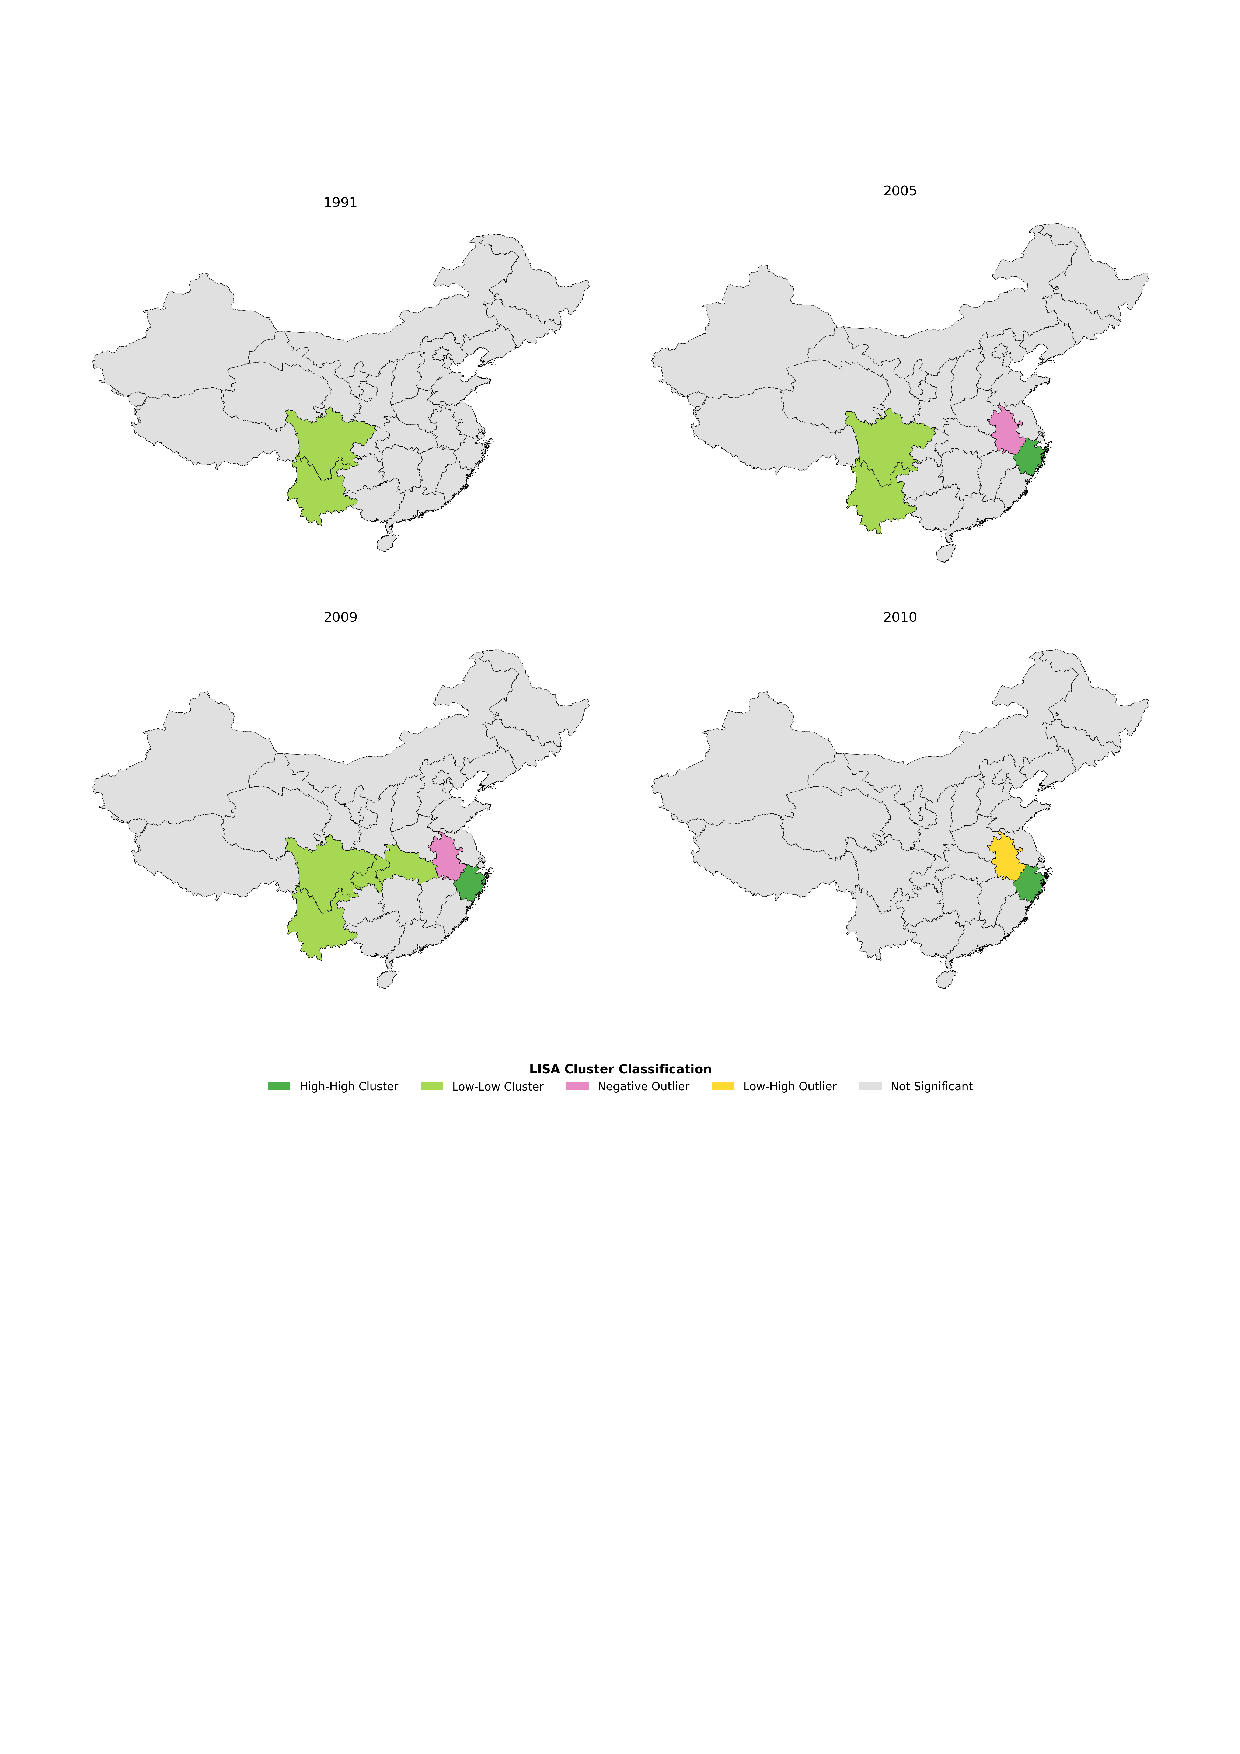
\includepdf[pages=1, scale=0.8]{china.pdf}
    \label{fig:china_map}
    \vspace{14cm}
    \caption*{Source: Compiled by the author.}
\end{figure}


Thus, Taiwan's investment in China over the past 20 years has been highest in the province of Zhejiang, which exhibited the strongest spatial correlation and greatest homogeneity with the surrounding areas. In contrast, Anhui province and its neighboring 16 areas demonstrated minimal spatial heterogeneity. The investment pattern of Taiwanese businesses in mainland China reveals polarization and a lack of an appropriate interregional cooperation mechanism, resulting in weak spatial correlation between regions, as noted by \cite{alves_ml_wald_tests}. The inter-regional distribution of Taiwanese investment has not fostered a more interactive development situation between both sides of the Strait, according to \cite{yeung_what_you_need_to_know_china_taiwan_tensions}.

Within this pattern of Taiwanese investments in China, significant sectors have been impacted by the island's strategic posture shift, as discussed by \cite{yeung_what_you_need_to_know_china_taiwan_tensions}. The results indicate that regional differences were not accounted for, and the most important factors in Taiwanese investment in mainland China over the past three years (2007, 2008, and 2010) include improvements in the natural environment, infrastructure, and economic risk (see Table ~\ref{tab:panel}).

\begin{table}[H]
\centering
\caption{Results of the General Analysis of the Panel Model}
\begin{tabular}{l S[table-format=-1.6] S[table-format=1.6] S[table-format=-1.6] S[table-format=1.4]}
\toprule
\textbf{Variables} & \textbf{Coefficient} & \textbf{Std. Error} & \textbf{t-Statistic} & \textbf{Prob.} \\
\midrule
ENVI   &  0.437815 & 0.465588 &  0.940349 & 0.0372 \\
INFR   & -1.134638 & 0.601653 & -1.885869 & 0.0595 \\
SOEN   &  2.189960 & 0.485041 &  4.514996 & 0.0000 \\
LAWE   & -6.714128 & 0.597710 & -11.23308 & 0.0000 \\
ECEN   &  4.732710 & 0.400019 &  11.83122 & 0.0000 \\
MARKE  &  8.004338 & 0.634303 &  12.61315 & 0.0000 \\
INEN   & -0.831210 & 0.417115 & -1.992758 & 0.0465 \\
SORI   &  2.888208 & 0.534176 &  5.406851 & 0.0000 \\
LARI   & -6.854205 & 0.750625 & -9.131328 & 0.0000 \\
MARI   &  4.887199 & 0.805937 &  6.063994 & 0.0000 \\
ECRI   &  0.001636 & 0.739322 &  0.002213 & 0.0982 \\
RECO   & -3.817749 & 0.426538 & -8.950542 & 0.0000 \\
\midrule
R\textsuperscript{2}           & 0.386220 & & & \\
Adj. R\textsuperscript{2}     & 0.381071 & & & \\
S.E. Regression & 1.421319 & & & \\
Residual sum of R\textsuperscript{2} & 2648.415 & & & \\
Durbin Watson test & 1.393557 & & & \\
Second Stage SSR & 2648.415 & & & \\
Instrument Rank & 13.00000 & & & \\
\bottomrule
\end{tabular}
\caption*{Source: Compiled by the author.}
\label{tab:panel}
\end{table}

The results indicate that several variables significantly affected Taiwanese investment in the Chinese market at the 5\% level. Among these factors, the social environment, economic environment, and market environment had significantly positive impacts. The legal environment and innovation environment exhibited significantly negative impacts. Social and market risks had significantly positive effects on investment in Taiwan, while legal risk had a significantly negative impact. The degree of preference for Taiwan also had a significantly negative effect. It can be concluded from these results that the factors that effectively promoted Taiwanese investment in mainland China over the past three years primarily include the social environment, economic environment, market environment, and reduced legal risk.

The results presented from the spatial error model with fixed effects (SEM) demonstrate that the 21 sampled areas receiving Taiwanese investment in 2008, 2009, and 2010 had effects in both the fixed spatial effects model and the temporal fixed effects model (see \ref{tab:SEM}). The geographic environment and market environment exhibited a significant positive relationship with Taiwanese investment at the 1\% level; infrastructure and the legal environment showed a significant negative correlation at the 1\% level; business risk and the appreciation level of Taiwanese entrepreneurs demonstrated a significant negative correlation at the 5\% level.


\begin{table}[H]
\centering
\caption{Fixed-effect spatial error model (SEM)}
\begin{tabular}{l S[table-format=-1.6] S[table-format=-1.6] S[table-format=-1.6] S[table-format=-1.6]}
\toprule
\textbf{Variables} & \multicolumn{4}{c}{\textbf{Coefficient}} \\
\cmidrule(lr){2-5}
 & \textbf{Model 1} & \textbf{Model 2} & \textbf{Model 3} & \textbf{Model 4} \\
\midrule
Intercepts & 11.7995 & & & \\
ENVI      & 1.3662 & 2.441638\textsuperscript{***} & 1.947974 & 2.946701\textsuperscript{***} \\
INFR      & -2.1184 & -4.711658\textsuperscript{***} & -2.075676 & -5.252975\textsuperscript{***} \\
SOEN      & 3.0410 & 1.912495\textsuperscript{*} & 3.760813\textsuperscript{*} & 1.856820\textsuperscript{*} \\
LAWE      & -7.4177\textsuperscript{***} & -4.003429\textsuperscript{***} & -8.309495\textsuperscript{***} & -4.377563\textsuperscript{***} \\
ECEN      & 4.5272\textsuperscript{**} & 0.969862 & 4.874697\textsuperscript{***} & 0.843587 \\
MARKE     & 7.1753\textsuperscript{**} & 4.465349\textsuperscript{***} & 6.916222\textsuperscript{**} & 5.001891\textsuperscript{***} \\
INEN      & -1.2589 & -2.188730\textsuperscript{**} & -1.527832 & -2.250578\textsuperscript{**} \\
SORI      & 1.7089 & 0.783276 & 1.417288 & 1.431297 \\
LARI      & -6.6332\textsuperscript{**} & -0.882737 & -7.455075\textsuperscript{**} & -0.703268 \\
MARI      & 3.3069 & -4.182716\textsuperscript{*} & 3.404127 & -5.666034\textsuperscript{**} \\
ECRI      & 0.6318 & 1.579397 & 1.568447 & 2.009705 \\
RECO      & -4.4494\textsuperscript{**} & -1.883895\textsuperscript{**} & -4.853772\textsuperscript{**} & -2.048145\textsuperscript{**} \\
Spat.aut. & -0.1790 & -0.210969 & -0.233976\textsuperscript{*} & -0.312971\textsuperscript{**} \\
\midrule
R         & 0.4145 & 0.9296 & 0.4075 & 0.9289 \\
F         & -110.08523 & -43.476101 & -110.68627 & -44.30271 \\
Total Time & 0.4810 & 0.1220 & 0.0970 & 0.1140 \\
\bottomrule
\end{tabular}
\vspace{0.5cm}
\caption*{Note: *p < 0.1; **p < 0.05; ***p < 0.01. Model 1: No fixed effects; Model 2: Spatial fixed effects; Model 3: Temporal fixed effects; Model 4: Spatial and temporal fixed effects.}
\caption*{Source: Compiled by the author.}
\label{tab:SEM}
\end{table}

The results from the spatial error model (SEM) indicated that differences in geographical and inter-regional market environments, along with gradual improvements in these factors across regions, had a significant positive impact on Taiwanese investments in mainland China over the past three years (2008, 2009, and 2010). 

Conversely, disparities in inter-regional infrastructure and the legal environment significantly constrained Taiwan's regional investment strategy. The results from Model 4 suggest that business risks and the level of appreciation among Taiwanese entrepreneurs notably (at the 5\% level) restricted the investment choice strategy of Taiwanese businesses in mainland China. If regional differences were not considered, the most important factors influencing Taiwanese investments in mainland China over the past three years—such as the social environment, economic environment, market environment, social risk, and market risk—could have had significantly greater positive impacts. Conversely, the legal environment, innovation environment, legal risk, and the level of appreciation among Taiwanese entrepreneurs had significantly negative effects on investment in Taiwan. 

In simple terms, Taiwan's major political events have influenced the convenience of investment in China, with a more democratic government returning to power, gradually diminishing the positive messaging favoring economic interaction across the Strait. This also affected and altered the confidence, behavioral strategies, and regional distribution of Taiwanese investments in mainland China. 

The lingering question remains: even as Taiwan may be investing more in certain Chinese areas or regions, while others experience reduced investments amidst China's increasingly hostile behavior towards Taiwan—stemming from beliefs of sovereignty over the Strait—will China indeed invade Taiwan? Moreover, will the United States protect Taiwan? In this conflict, what may be more critical: political or economic considerations? Given that Taiwan is economically intertwined with both China and the United States, as evidenced by a gradual decline in its investments in mainland China over the past 20 years \citep{pietrafesa_political_economic_relations_china_taiwan_usa}.

\section{Will China Invade Taiwan? Will the Americans Protect the Island? Will Politics or Economics Prevail in this Conflict?}

Following the qualitative and statistical discussion, it appears that China is increasingly close to launching an offensive against Taiwan. From this perspective, several motivations can be identified regarding a potential Chinese invasion of the island:

\begin{itemize}
    \item \textbf{The Westernization of Taiwan} is a significant factor. As previously discussed, relations between Taipei and Beijing have become increasingly tense since the election of President Tsai Ing-wen in January 2016. Xi Jinping perceives the new democratic government in Taiwan, which aligns more closely with American policies and distances itself from the One China policy, as a threat to the stability of both sides of the Strait and the dream of national rejuvenation in China. This is in stark contrast to the era of Ma Ying-jeou, who, despite adopting the One China policy, had high levels of military procurement from the United States, thereby modernizing Taiwan's military as a means of self-defense against China.
    \item \textbf{The military modernization of Taiwan} poses an ongoing challenge to Chinese aspirations. The continuous export of U.S. arms to Taiwan has bolstered the Taiwanese public’s sentiment towards independence, enhancing their desire to assert sovereignty in the region. This military support serves as a countermeasure to China's national rejuvenation policy.
    \item \textbf{President Tsai's opposition to the One China policy} complicates matters further. She refuses to recognize the 1992 Consensus, which asserts that both Taiwan and the mainland are part of "one China." Tsai maintains that the Taiwanese should be considered an independent state, which eliminates the need for a formal declaration of independence. Her efforts to seek greater international recognition align with the sentiments of the Taiwanese populace, a majority of whom do not support the idea of both sides of the Strait belonging to "one China." Furthermore, her administration has worked to enhance American presence on the island, with notable visits from high-ranking U.S. officials, showcasing strong support for Taiwan's democratic government.
    \item \textbf{The support from the West for Taiwan remains crucial.} The primary priority for Americans in the event of a Chinese invasion would be to support Taiwan, a trend that has persisted for decades. Western backing manifests through military modernization, increased international engagement for Taiwan, and public support against Chinese aggression. However, should China seize Taiwan, it could unleash significant military resources to protect itself against a potential American invasion, escalating the conflict's costs and potentially dissuading U.S. intervention despite strong declarations of military support for Taiwan.
    \item \textbf{There is a noticeable reduction in China’s economic share in Taiwan.} Despite ongoing American support, Taiwan remains economically dependent on China, which is its largest trading partner. The refusal of Tsai to adopt the One China policy indicates Taiwan’s gradual attempt to decouple its economy from China. For instance, there was a symbolic decrease in China’s market share in Taiwan from 2017 to 2019. This trend highlights a shift, even though China had previously increased its economic influence in Taiwan significantly from 2000 to 2008.
    \item \textbf{Lastly, there is a decline in Taiwanese investments in China.} The investments made by Taiwan in mainland China are negatively correlated with commercial risks, illustrating that economic and political relations between the two countries have influenced Taiwan's investment strategies. The rising tensions, whether political or economic, have altered Taiwanese behavioral strategies and regional investment distribution.
\end{itemize}

In conclusion, despite the outlined motivations, it remains difficult to estimate the likelihood of a short-term invasion of Taiwan, as China stands to lose more than it gains from such a conflict. For example, given China's extensive trade ties with countries like Japan and Korea, which have strong Western influence, retaliatory actions against China could result in severe economic difficulties. Furthermore, American military cooperation with Western-aligned states in Asia could hinder Chinese advances against Taiwan, significantly increasing the costs of any military conflict.

While the aggressive postures of Xi Jinping toward Taiwan are evident, and the Chinese state's doctrine often emphasizes the use of force, it remains uncertain if Taiwan will continue Tsai's policies in the long term. If so, the possibility of a forced invasion by China may become more pronounced in the future.

\section{Final Considerations}

This research project examined the levels of tensions—both in security and economic and econometric terms—among the United States, China, and Taiwan. The empirical studies showed divergent results on this topic. The project's findings clearly indicated that the United States (U.S.) has maintained a dual alignment policy with both sides of the Taiwan Strait since the Obama administration. Furthermore, China is motivated to use force to achieve reunification with Taiwan if it continues to delve deeper into Western politics \citep{huang_xi_jinping_taiwan_policy}.

These observations have important implications for the Chinese offensive in the region and for the United States. The U.S. commitment to Taiwan's security, particularly the continuation of arms sales to Taiwan, represents one of the main sources of tension in the broader Sino-American relationship. In recent years, analysts in both Washington and Beijing have proposed new approaches to the issue \citep{haass_sacks_american_support_taiwan}. In the United States, some have suggested that the country should cease arms sales to Taiwan and consider withdrawing its commitment to the island more broadly. In the People's Republic of China (PRC), some have suggested that a rising China should adopt a harder line in response to U.S. arms sales \citep{haass_sacks_american_support_taiwan}.

It is evident that both proposed political alterations carry significant risks. In the case of the U.S., ending arms sales or trade relations with Taiwan could increase the likelihood of conflict in the Strait, shifting relations between the two sides from a deterrence dynamic to a competition dynamic \citep{lee_siu_taiwan_leader_hawaii_stopover}. In the Chinese case, a tougher approach to U.S. arms sales and trade could have the opposite effect, revealing a stronger U.S. commitment to Taiwan's security than might currently be assumed \citep{panda_taipei_slams_chinese_air_force_fighters}.

In other words, Taiwan's increasing proximity to the United States (the West) infuriates the Chinese, who attempt to isolate the island from the rest of the world \citep{wenzhao_taiwan_policy_obama_administration}. The dream of national rejuvenation involves unification with the island, and no power will separate both sides of the Strait \citep{silk_is_taiwan_part_of_chinese_dream, xinhua_xi_steadfast_on_reunification}.

Finally, the research project demonstrates that although the United States is attempting to integrate Taiwan into more international affairs—whether political, security, or trade—China remains steadfast in its stance and considers an offensive against the rebellious island. To achieve the Chinese dream, reunification with the rebellious society, namely Taiwan, must come first \citep{huang_xi_jinping_taiwan_policy}.

\bibliographystyle{apalike}
\bibliography{references}

\end{document}